\section{Gruppierte Erkenntnisse bezüglich der API-Usability-Forschung}
\label{sec:forschung-einzelne-ergebnisse}

In diesem Abschnitt fasse ich Ergebnisse der API-Usability-Forschung in logische Gruppen zusammen. Ich beschränke mich dabei auf die Arbeiten, die ausreichend verallgemeinerbare Erkenntnisse vorstellen und für meine Forschung von Relevanz sind.

Arbeiten, die ich im Folgenden nicht weiter betrachte, befassen sich mit statischer und dynamischer Typisierung \citep{Mayer:2012kl}, Kapselung \citep{Schmidt:br,Roberts:1997tt,Stylos:2008jt,Piccioni:2013uq} sowie Sichtbarkeit, Abwärtskompatbilität, Interoperabilität, Nebenläufigkeit und Wartung \citep{Zibran:2011fx}, API-Evolution \citep{Ng:2007gh} und Speicherverbrauch \& Kosten \citep{Henning:2007kg}.


%\subsection{Abstraktionsmöglichkeiten}

%Über je mehr syntaktische und semantische Kenntnisse ein Anwender verfügt, desto besser kann er Quellcode verstehen, indem er einfachen Anweisungen zu komplexen abstrahiert \citep{BenShneiderman:gn,Shneiderman:1977jj}. Dies fördert das Einprägen des Programms, was nach \citep{Shneiderman:1977jj} mit einem besseren Verständnis korreliert.
  
%Semantisches Wissen kann genutzt werden, wenn Entwickler dem Anwender bekannte Konzepte verwendet. \citep{BenShneiderman:gn}
  
%Die Wichtigkeit syntaktischen Wissens ist für meine Arbeit insofern relevant, als das SeqAn, wegen einer grundlegenden Entwurfsentscheidung, eine unübliche Syntax verwendet.
  
%Das Programmverständnis kann durch die Bereitstellung einer abstrakten Dokumentation der zentralen Entwurfsentscheidungen verbessert werden. \citep{Robillard:2009cs}
  
%Zweckdienlich sind ebenso ``high-level''-Kommentare. ``low-level''-Kommentare fördern im besten Fall nur geringfügig das Verständnis, weil sich lediglich den Quellcode paraphrasieren. \citep{BenShneiderman:gn}
    
%Opportunistische Entwickler haben größere Probleme beim Debuggen haben, wenn sich das zu lösende Problem über mehrere Objekte erstreckt. \citep{Stylos:2007jb}
  
  
\subsection{Dokumentation}

  Die meisten \citep{Zibran:2011fx,Grill:2012jm} bzw. dramatischsten \citep{Robillard:2010bh} bzw. fundamentalsten \citep{Bloch:2006jk} API-Usability-Probleme rühren von der API-Dokumentation her.
  
  Eine Ursache liegt in der Verwendung verschiedener Bezeichnungen für dasselbe Konzept \citep{Aguiar:2000dn}, was auch als \textit{Vocabulary Problem} bekannt ist \citep{Good:1984kr,Furnas:1987hl}. Im Kontext von Dokumentationen eignet sich die Unterstützung von Aliassen \citep{Stylos:2009gc}, also Platzhaltereinträgen, die auf den korrekten Eintrag verweisen.
  
  Weitere Ursachen sind ein inkonsistentes Aussehen, fehlende grafische Darstellungen, sowie schlechte Navigations- und Suchfunktionen. \citep{Jeong:kf}
  
  Eine benutzerfreundliche Dokumentation verfügt über Beispiele, Best-Practise-Beispiele, Erläuterungen der Entwurfsentscheidungen \citep[ebenso ][]{Aguiar:2000dn}, einen zielgruppenspezifischen API-Überblick \citep[ebenso ][]{Fairbanks:2006jw,Ko:2011vw,Pugh:Ks4cicwp,Nykaza:2002im}, Erläuterungen zu komplexen Anwendungsszenarien und eine durchdachte Organisation. \citep{Robillard:2009cs}
  
  Existenziell wichtige Begriffe müssen erklärt werden --- unabhängig von den angenommenen Vorkenntnissen der Anwender. \citep{Jeong:kf,Nykaza:2002im}

  Eine gute Form der Gruppierung ist die logische Gruppierung. Eine alphabetische Sortierung, wie sie bei JavaDoc zum Einsatz kommt, zwing den Anwender mental selbst eine Gruppierung vorzunehmen. \citep{DaqingHou:2005ba}
  
  Der Dokumentationstext selbst muss einen klaren Fokus haben, Direktiven nennen und keine vagen Formulierungen (z.B. ``sollte'') verwenden \citep{Monperrus:2011bf}. Außerdem muss er präzise, vollständig und aktuell sein \citep{Piccioni:2013uq,Parnas:2011kr,Zibran:2011fx}.
  
  ``Die schlechteste Person zum Schreiben der Dokumentation ist der Implementierer und der schlechteste Moment, eine Dokumentation zu schreiben, ist nach der Implementierung.'' \citep{Henning:2007kg}
  
  
  
\subsection{Tutorials}
  
  Tutorials stellen eine Spielart des ``Fact Findings'' \citep{LaToza:2007fj} dar (siehe \sref{sec:FactFinding}) und helfen beim Erlernen einer API \citep{McLellan:1998cu}.
  
  Tutorials stellen eine Möglichkeit dar, den von \cite{Robillard:2010bh} geforderten API-Überblick zu geben \citep{Nykaza:2002im}. Deren Verlinkung auf der Startseite der Dokumentation ist verpflichtend \citep{Watson:2012es}.
  
  Tutorials erlauben die Darstellung der von \cite{Robillard:2009cs} geforderten, komplexen Anwendungsszenarien \citep{DaqingHou:2005ba}.
  
  Tutorials erleichtern die Anwendung der \textit{flexiblen Programmverständnisstrategie}.\footnote{Darunter wird der bedarfsabhängige Wechsel zwischen Top-Down- und Bottom-Up-Vorgehen verstanden.} \citep{Shaft:1998tc}
  
  Ohne die Bereitstellung von Tutorials wird der Einstieg in neue API stark erschwert. \citep{DaqingHou:2005ba}
  

\subsection{Beispiele}
  
  Beispiele sind notwendiger Bestandteil einer lernförderlichen Dokumentation \citep{Tenny:1988ir,Jeong:kf,Shull:2000fy,McLellan:1998cu,Nykaza:2002im}. Sie erlauben die Verknüpfung von abstrakten und konkreten API-How-To-Wissen \citep{Shaft:1998tc}.
  
  Jeder nicht-triviale Dokumentationseintrag benötigt ein Beispiel. \citep{DaqingHou:2005ba}
  
  Es gibt eine Reihe an Werkzeugen (siehe \sref{sec:api-tools}), welche die Bereitstellung von Beispielen erleichtern.
  
  Je geringfügiger Anwender kopierten Beispielcode an ihren ``Anwendungskontext'' anpassen, desto größer ist die Wahrscheinlichkeit, dass die Anwender den Code nicht verstanden haben. Wird der Code mittels Debugging angepasst, wird dies als ``debugging into existence'' bezeichnet. \citep{Rosson:1996da}

  Für Anwender des Bottom-Up-Vorgehens (siehe Abschnitte \ref{sec:bottomup} und \ref{sec:shaft}), sind konkrete Beispiel existenziell. \citep{Rosson:1996da}
  
  Bei optimistischen Entwicklern birgt die Bereitstellung von Beispielen die Gefahr der \textit{Verständnisvermeidung} \citep[siehe \sref{sec:Verstandnisvermeidung},][]{Rosson:1996da,Stylos:2008jt}.
  

\subsection{Benennung}
\label{sec:naming}

Sinnlose Variablennamen erhöhen die Komplexität des Verständnisprozesses \citep{BenShneiderman:gn} und verschlechtern die User Experience\footnote{In der Studie von \cite{Blinman:2005wr} mussten die Probanden an Programmen mit einer schlechten Benennung arbeiten. Festgehaltene Aussagen waren ``This sucks!'', ``I'm getting lost.'' und ``These are filthy names.''} \citep{Blinman:2005wr}.

Sinnvolle Variablen- und Funktionsnamen dienen als \textit{Beacons} (siehe \sref{def:beacon}) und beschleunigen den Verständnisprozess. \citep{Gellenbeck:1991vn}

Funktionsnamen sollten die Lösung und nicht die Implementierung beschreiben und bei einer booleschen Rückgabe  eine aktive Stimme verwenden. Idealerweise ergibt eine Programmzeile einen Satz.\footnote{Beispiel: \mintinline{java}{if(!isValid())} statt \mintinline{java}{if(!valid())}} \citep{cwalina2008framework}

Die Beziehungen zwischen Konzepten sollten sich im Namen widerspiegeln. \citep{cwalina2008framework,Watson:2009da}

Deskriptive Namen sind abgekürzten Namen vorzuziehen \citep{Zibran:2011fx}, allerdings führen zu lange Namen  in der Wahrnehmung zu einem ``blinden Fleck'' (engl. \textit{blind spot}). Dieser führt wiederum dazu, dass Anwender nur noch Anfang und Ende des Bezeichners wahrnehmen. \citep{Beaton:2008jn}

Nicht die abstrakte Klasse, sondern die am häufigsten verwendete Unterklasse sollte den prägnanten und kurzen Namen erhalten\footnote{Negatives Beispiel: Oberklasse = ``Message'', Unterklasse: ``MimeMessage''} \citep{Stylos:2008jt}.

Eine Benennung, die nah an der Anwendungsdomäne ist, verbessert das API-Verständnis \citep{BenShneiderman:gn,Tenny:1988ir,Teasley:1994gr,Briand:1997fw,Jeong:kf}. Dabei muss sie konzeptionell korrekt sein \citep{Zibran:2011fx}.

Umgekehrt wird das Verständnis verschlechtert, wenn die Benennung technisch getrieben ist, also eine Variable beispielsweise \texttt{integerArray} heißt \citep{Teasley:1994gr}. Zu einer Verschlechterung kommt es auch, wenn semantisch überladene Begriffe (z.B. ``template''\footnote{Abhängig von der Anwendungsdomäne könnte es sich um einen fachlichen Begriff handeln. Kommt die Programmiersprache C++ zum Einsatz, würde es zu einer semantischen Überladung kommen, weil nicht eindeutig ist, ob der Begriff fachlich oder technisch gemeint ist.}) verwendet werden \citep{Gellenbeck:1991vn}.

Wissenschaftliche Erkenntnisse zum Thema komplexer Anwendungsdomänen konnte ich nicht finden. Eine den Anwendungsdomänen nahe Benennung ist anspruchsvoll, wenn es spezielle Teildisziplinen gibt (z.B. \textit{CRUD}-Operationen im Datenbankbereich), oder das Fach selbst fachübergreifend ist (z.B. Bioinformatik, Wirtschaftsinformatik). Ebenso ergibt sich ein Problem, wenn die Anwenderschaft aus zwei unterschiedlichen Gruppen, z.B. Informatiker und Wirtschaftsexperten, besteht \citep{Jeong:kf}. Auf diese Beobachtung werde ich im \sref{sec:Ergebnisse} näher eingehen.

Namen müssen verständlich, konsistent \citep[auch ][]{Briand:1997fw,Zibran:2011fx,McLellan:1998cu} und symmetrisch\footnote{Diese Eigenschaft ist am besten mit einem Beispiel erklärt: Wenn es die Funktionspaare (\mintinline{java}{keySet()}; \mintinline{java}{hasKey(Object)}) und (\mintinline{java}{values()}; \mintinline{java}{hasValue(Object)}) gibt, muss es auch für die Funktion \mintinline{java}{entrySet()} das symmetrische Pendant \mintinline{java}{containsEntry(V, K)} geben. Javas \texttt{Map}-Interface verletzt also diese Forderung.} sein. \citep{Bloch:2006jk}

Das \textit{Vocabulary Problem} \citep{Good:1984kr,Furnas:1987hl} erschwert eine gute Benennung. Das Problem sollte nicht in der API selbst, sondern in dessen Dokumentation gelöst werden \citep{Stylos:2009gc}. Auf eine technische Lösung gehe ich unter in den Abschnitten \ref{sec:Jadeite} und \ref{sec:improve-dox} ein.

Eine gute Benennung verbessert die API-Anwendung \citep{Bloch:2005wn} und verringert die Konsultation der Dokumentation \citep{Blinman:2005wr}.

Eine schlechte Benennung führt dazu, dass die Verwendung der Dokumentation dramatisch ansteigt. Ist auch die Dokumentation schlecht, sinkt die Performanz. \citep{Blinman:2005wr}

Erfahrene Entwickler werden von einer schlechten Benennung weniger beeinflusst als Anfänger \citep{Blinman:2005wr,Teasley:1994gr,Crosby02theroles}, denn fortgeschrittene Enwickler verfügen über mehr Erfahrung \citep{Teasley:1994gr} und können ein größeres Spektrum an Beacons erkennen. Dadurch sind sie nicht allein auf die Beacons \textit{naming style} und \textit{documentation} angewiesen \citep{Crosby02theroles}.



\subsection{Konsistenz}

Ein konsistenter Entwurf, der etablierten Konventionen folgt, erhöht die API-Usability. \citep{Zibran:2011fx}

Immer mehr \glslink{api}{APIs} verwenden das \textit{create-set-call}-Muster als Alternative zu Konstruktoren mit Parametern. Daher sollten Entwickler beim Entwurf einer API das \textit{create-set-call}-Muster vorziehen \citep{Stylos:2007jb}. Konstruktoren, die sich auf die wichtigsten Parameter beschränken, um ein invariantes Objekt zu erzeugen, stellen eine vertretbare Alternative zu parameterlosen Konstruktoren dar \cite{Piccioni:2013uq}.

Die Benennung innerhalb einer API muss konsistent sein \citep{Bloch:2006jk,Briand:1997fw,Zibran:2011fx,McLellan:1998cu}.

Je höher der API-interne Konsistenz ist, desto kritischer wirken sich ungewollte Inkonsistenten aus. Anwender vermuten hinter ihnen häufig bewusste Design-Entscheidungen. \citep{Watson:2009da}


\subsection{API-Entwurf}

Die Anzahl und die Typen von Funktionsparametern haben einen signifikanten Einfluss auf die API-Usability. Zu viele Parameter beeinflussen sie nachteilig. Das Gleiche gilt für Parameter, die schwierig zu konstruieren sind. \citep{Zibran:2011fx}

Mechanismen, die den kontrollierten Umgang mit Versagenssituationen erlauben, verbessern die Usability. Ebenso verhält es sich, wenn Diagnoseinformationen bereitgestellt werden. \citep{Zibran:2011fx}

Lösungswege sollten eindeutig sein. Alternative Lösungsoptionen, die das Gleiche tun, führen zu Verwirrung und verschlechtern die API-Usability. \cite{Piccioni:2013uq,Zibran:2011fx}



\subsubsection{Fabrikmethode}

Die Autoren der qualitativen Studie ``The Factory Pattern in API Design: A Usability Evaluation'' \citep{Ellis:2007kv} haben mit einem Experiment, bei dem 12 Probanden Programmieraufgaben in Java lösen sollten, die Auswirkungen des Fabrikmusters auf die API-Usability untersucht.

\cite{Ellis:2007kv} fanden heraus, dass die API-Anwender viel mehr Zeit zur Konstruktion eines Objekts mit Hilfe des Fabrikmusters benötigten als mit klassischen Konstruktoren. Sie beobachteten, wie die API-Anwender bei der Abwesenheit von Konstruktoren in der Klasse eher nach Unterklassen mit Konstruktoren suchten. Andere Probanden probierten --- meist erfolglos --- selbst einen Konstruktor zu schreiben.

Ergebnis der durchgeführten Interviews war, dass die Probanden das Fabrikmuster nur dann präferierten, wenn es sich um die Konstruktion von unveränderlichen Objekten ohne Operationen handelt (\textit{opaque objects}).

Die Autoren stellen in ihrer Arbeit außerdem objektive Probleme des Fabrikmusters vor. Dazu gehört die Notwendigkeit einer abstrakten Fabrik, sämtliche konkrete Implementierungen zu kennen. Allein das Finden einer Fabrik ist ebenfalls ein Problem. So ist es in .NET üblich, mit einer Fabrik Objekte verschiedener Typen zu erzeugen, während es bei Java häufig die Suffixregel gibt, bei der die zu einem Typ \texttt{Type} gehörige Fabrik \texttt{TypeFactory} lautet.

\cite{Ellis:2007kv} schließen aus ihren Ergebnissen, dass sich die Verwendung der Fabrikmethode deutlich negativ auf die API-Usability auswirkt. Alternativen wie der klassische Konstruktor oder das \textit{Class Cluster}\footnote{\url{http://www.uow.edu.au/~nabg/ASWEC96/aswec96.html}} sind unbedingt der Fabrikmethode vorzuziehen.


\subsubsection{Konstruktoren}

\cite{Stylos:2007jb} haben sich mit der Frage befasst, inwiefern sich Konstruktoren, die Parameter verlangen, auf die API-Usability auswirken.

Dazu führten sie ein Experiment durch, bei dem 30 professionelle Entwickler verschiedene Programmieraufgaben in Visual Basic, C\# und C++ lösen mussten. Im Anschluss an die Programmieraufgaben wurden Interviews mit den Teilnehmern durchgeführt.

Für die Konstruktion von Objekten gibt es grundsätzlich zwei Ansätze:
\begin{description}
  \item[Konstruktoren mit Parametern] Bei dieser Variante wird ein Konstruktor mit einer endlichen Anzahl von Parametern aufgerufen, um ein Objekt zu erzeugen.
  \item[Standard-Konstruktor] Bei dieser Variante wird der parameterlose Standardkonstruktor aufgerufen --- gefolgt von endlichen vielen \texttt{set}-Aufrufen. Diese Variante wird von den Autoren auch als \textit{create-set-call pattern} bezeichnet.
\end{description}

Die Forscher fanden heraus, dass der Gebrauch des \textit{create-set-call}-Musters zu weniger Fehlern in der Anwendung führte. Dies ist insoweit erstaunlich, als dass sich ein Objekt, das mit einem Standardkonstruktor instanziiert wurde, ohne darauf folgende \texttt{set}-Aufrufe in einem potentiell inkonsistenten Zustand befinden und zu weiteren Anwendungsschwierigkeiten führen kann.

Die Erkenntnisse wurden nach den Personas von Clarke \cite[][siehe \sref{sec:personas}]{clarke:DSP:2007:1080} aufgeschlüsselt:
\begin{description}
  \item[Opportunistischen Entwicklern] kommt das \textit{create-set-call}-Muster am meisten entgegen, denn bei ihnen besteht ein ausgeprägter Fokus auf das Erreichen des Ziels. Die Erklärung ist so einfach wie wichtig. Die analysierten opportunistischen Entwickler wollten zunächst herausfinden, ob sie mit dem korrekten Objekt arbeiten, um dann zu prüfen, welche bereitgestellte Methode die Aufgabe löst (siehe \fref{fig:CreateAndUseObjectMode}). Für die Exploration der Methoden musst das Objekt jedoch erst konstruiert werden. Bei Konstruktoren mit Parametern konnte dieser Prozess sehr aufwendig sein, da unter Umständen auch diese Parameter über Konstruktoren mit Parametern verfügten, was zu einem rekursiven Konstruktionsprozess führt. Und das ``nur'', um die Frage zu klären, ob man es überhaupt mit dem korrekten Objekt zu tun hat.
  \item[Pragmatische Entwickler] empfanden den Gebrauch des \textit{create-set-call}-Musters als weniger störend und geradliniger.
  \item[Systematische Entwickler] favorisierten --- zur Überraschung der Forscher --- das \textit{create-set-call}-Muster, da es eine höhere Flexibilität bietet. Diese Persona hatte mit keiner der beiden Konstruktionsvarianten Anwendungsschwierigkeiten.
\end{description}

\begin{figure}
  \centering
    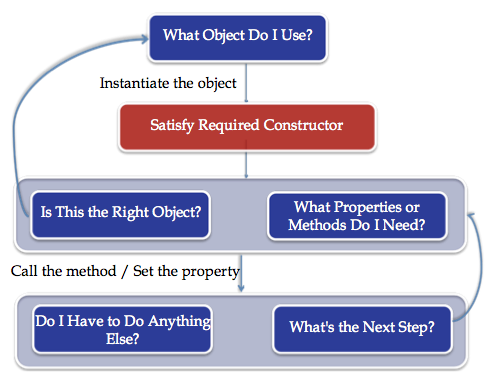
\includegraphics[width=0.6\linewidth]{Figures/CreateAndUseObjectMode.png}
    \caption[Problemlösung bei Verwendung von Konstruktoren mit und ohne Parametern]{Wenn Konstruktoren mit Parametern verwendet werden müssen und es dabei zu Problemen kommt (insbesondere IDE-Kompilierfehlern), führt dies zur Unterbrechung des Explorationsprozesses. Der API-Anwender muss den Konstruktor zunächst korrekt verwenden, bevor er fortfahren kann. \citep{Stylos:2007jb}}
    \label{fig:CreateAndUseObjectMode}
\end{figure}

Entlang der \glslink{cd}{kognitiven Dimensionen} von Clarke \cite[][siehe \sref{sec:api-cds}]{Anonymous:9HSMlhmF} fassen die Forscher die Ergebnisse der Interviews und ihrer Beobachtungen wie folgt zusammen:
\begin{description}
  \item[Work-Step Unit] Die Work-Step Unit\footnote{Inkonsistenter Weise werden in der Arbeit die ursprünglichen kognitiven Dimensionen \citep{Green:1989wb} mit denen für die Evaluation von APIs \citep{Anonymous:9HSMlhmF} vermischt, denn die Forscher sprechen sowohl von \textit{Work-Step Unit} als auch von \textit{Diffuseness}. Im \sref{sec:api-cds} habe ich bereits meine Kritik an Clarks kognitiven Dimensionen geschildert.} wird objektiv durch den Gebrauch von Konstruktoren mit Parametern vergrößert. Das bedeutet, es wird weniger Code für die Erledigung einer konstanten Arbeit benötigt. Umgekehrt benötigt das \textit{create-set-call}-Muster mehr Code, was sich aber laut der Forscher  nicht negativ auf die Lesbarkeit des Codes auswirkt.
  \item[Premature Commitment] Diese Dimension wird verstärkt, d.h. der API-Anwender muss zu einem frühen Zeitpunkt Dinge erledigen, die sich nicht auf seinem präferierten Lösungsweg befinden. Das \textit{create-set-call}-Muster erlaubt eine höhere Flexibilität bei der Konstruktion von Objekten.
\end{description}

Ein weiterer Vorteil des \textit{create-set-call}-Musters besteht in der differenzierten Fehlerbehandlung. In diesem Fall kann jede \texttt{set}-Methode spezifische Ausnahmen werfen, die bei einem Konstruktor mit Parameter zusammengefasst werden müssten.\footnote{Dieser Aspekt wird von der Greenschen kognitiven Dimension \textit{Error-Proneness} erfasst, die in Clarks CD fehlt und wahrscheinlich deswegen nicht im Rahmen der kognitiven Dimensionen erläutert wurde.}

Die Forscher resümieren, dass die Implementierung des \textit{create-set-call}-Musters der Implementierung von Konstruktoren mit Parametern vorzuziehen ist.

\cite{Piccioni:2013uq} stimmen den Erkenntnissen von \cite{Stylos:2007jb} weitgehend zu, geben dem Argument der Invariante aber ein größeres Gewicht. Sie kommen zu dem Schluss, dass auch Konstruktoren, die sich auf die absolut wichtigsten Parameter beschränken, um einen invarianten Zustand herzustellen, legitim sind.





\subsubsection{Platzierung von Methoden}
\label{sec:method-placement}

\begin{important}
\textit{Diese Arbeit ist besonders relevant für einige von mir in \href{sec:Ergebnisse}{Kapitel 4} vorgestellte \code{apiua://code/-9223372036854775414}, die ich bei den SeqAn-Anwendern beobachten konnte.}  

Vereinfacht ausgedrückt, hat sich die Arbeit ``The implications of method placement on API learnability'' von \cite{Stylos:2008jt} mit der Frage auseinandergesetzt, wie sich die Entwurfsalternativen \mintinline{java}{server.send(message)} und \mintinline{java}{message.send(server)} auf die Erlernbarkeit einer API auswirken.

Dazu wurden zehn Probanden dazu aufgefordert, Programmieraufgaben in Java zu lösen. Zuvor jedoch sollten die Probanden Pseudo-Code schreiben, um auf die Erwartungen der Probanden schließen zu können.

Die Autoren fanden heraus, dass das Zusammenspiel verschiedener Objekte grundsätzlich eine Herausforderung darstellen. Grundsätzlich vermuteten die Probanden die für die Aufgabe notwendige Methode in der so genannten \textit{Anfangsklasse} (engl. \textit{starting class}). Dabei handelt es sich um die Klasse, die nach dem Problemverständnis der Probanden die für die Lösung notwendige Methode bereithält. Die Beziehung zwischen Klasse und Methode wird als \textit{method ownership} bezeichnet.

So selbstverständlich diese Strategie klingen mag, so unerwartet sind die möglichen Probleme, auf welche die API-Anwender treffen:
\begin{enumerate}
  \item Eine ungünstige Benennung der Anfangsklasse erschwert dessen Auffinden enorm.
  \\Beispiel: Im Kontext von E-Mails ist es wahrscheinlich, dass die API-Entwickler für die Oberklasse die Bezeichnung ``Message'', und für die Unterklasse die Bezeichnung ``MimeMessage'' gewählt haben. Die Autoren haben jedoch beobachtet, dass die Probanden ``Message'' als die zu verwendende Klasse vermuteten, obwohl die ``MimeMessage''-Unterklasse notwendig war.
  \item Findet der API-Anwender keine relevante Funktion in der Anfangsklasse, tritt Verwirrung auf.
  \item API-Anwendern fällt es schwer, auf die Notwendigkeit einer zweiten \textit{Helferklasse} zu schließen, da sie davon ausgehen, dass nur eine Klasse notwendig ist.
  \item Das Auffinden der benötigten Helferklasse fällt den API-Anwendern schwer.
  \item Unsichtbare Abhängigkeiten sind extrem kritisch.
  \\Beispiel: Im Kontext des E-Mailversands in Java wird der Server nicht mit einer entsprechenden \mintinline{java}{message.setSmtpServer}-Methode gesetzt. Stattdessen muss ein \mintinline{java}{Options}-Objekt erzeugt werden, das eine solche Methode bereitstellt. Dieses wird dann mittels \mintinline{java}{message.setOptions(options)} an die Nachricht übergeben.
\end{enumerate}

Es konnte gezeigt werden, dass die korrekte Benennung der Anfangsklasse und die Platzierung der notwendigen Methode in dieser Anfangsklasse die Entwicklung mit der API um ein Vielfaches beschleunigt.

Den Autoren ist bewusst, dass diese beiden Anforderungen nicht immer zu erfüllen sind. Andere wichtige API-Anforderungen wie Performanz oder das \textit{Vocabulary Problem}\citep{Furnas:1987hl} können der kanonischen Lösung im Weg stehen. Eine verbesserte Dokumentation kann in solchen Fällen helfen. So ist es nicht nur möglich, Aliasse für Klassen, sondern auch Aliasse für Methoden in der Dokumentation zu pflegen. Beispielsweise könnte es einen Aliasseintrag für \mintinline{java}{Server.send(Message)} geben, der auf \mintinline{java}{Message.send(Server)} verweist.

Die Auffindbarkeit von Klassen halten die Autoren für existenziell und schlagen vor, für die Darstellung von Klassennamen in der Dokumentation unterschiedliche Schriftgrößen abhängig von ihrer Wichtigkeit zu verwenden.

Für meine Forschung sind die Erkenntnisse von \cite{Stylos:2008jt} besonders interessant. Während meiner Forschung zeigte sich, dass praktisch die gesamte Funktionalität von SeqAn durch globale Funktionen bereitgestellt wird. Das Konzept von \textit{method ownership} existiert in SeqAn zwar logisch, aber nicht technisch, was neue Probleme der Auffindbarkeit aufwirft.
\end{important}